% !TEX TS-program = pdflatex
% !TEX encoding = UTF-8 Unicode

% Example of the Memoir class, an alternative to the default LaTeX classes such as article and book, with many added features built into the class itself.

%\documentclass[12pt,a4paper]{memoir} % for a long document
\documentclass[11pt,a4paper,article]{memoir} % for a short document
\raggedbottom
\raggedright

\usepackage[utf8]{inputenc} % set input encoding to utf8
\usepackage{graphicx}
\usepackage{amsmath}
\usepackage{caption}
\usepackage{float}
\usepackage{parskip}
\usepackage{mathpazo}
\setlength{\parskip}{\baselineskip}%
\setlength{\parindent}{0pt}%

%%% PAGE DIMENSIONS
% Set up the paper to be as close as possible to both A4 & letter:
\settypeblocksize{*}{13cm}{1.8} 
\setulmargins{*}{*}{1} % 50pt upper margins
\setlrmargins{*}{*}{1}% golden ratio again for left/right margins
\setheaderspaces{*}{*}{1.618}
\checkandfixthelayout 
% This is from memman.pdf

%%% ToC (table of contents) APPEARANCE
\maxtocdepth{subsection} % include subsections
\renewcommand*{\cftappendixname}{Appendix\space}

%%% HEADERS & FOOTERS
\pagestyle{plain} % try also: empty , plain , headings , ruled , Ruled , companion

%%% CHAPTERS
\chapterstyle{section} % try also: default , section , hangnum , companion , article, demo

%%% SECTIONS
\hangsecnum % hang the section numbers into the margin to match \chapterstyle{hangnum}
\maxsecnumdepth{subsection} % number subsections


\makeatletter
\renewcommand\tableofcontents{%
\null\hfill\textbf{\huge\contentsname}\hfill\null\par
  \vspace{14pt}
  \@mkboth{\MakeUppercase\contentsname}{\MakeUppercase\contentsname}%
  \@starttoc{toc}%
}

\renewcommand\contentsname{Table of Contents}

\makeatother

\renewcommand{\baselinestretch}{1.5} 

\graphicspath{{./images/}}


%% RUBRIC %%%%%%%%%%%%%%%%%%%%%%%%
% Style pointers
% > Write in the past tense
% > Passive
% > 'Each paragraph should contain a complete thought or argument'

% RUBRIC
% ---------------------------------------------------------------------------------
% Communication
% 	> Abstract
% 	> Clear statement of aims/objectives
% 	> Overall quality of report:
%		- Structure
%		- Appearance
%		- Use of English
%		- Grammar
%		- Typographical errors
%		- Nomenclature
%		- Symbols
%		- Acronyms
%		- References
% 	> Introduction to process/method
% 	> Background of industry/company context
% 	> Presentation and discussion of work and results
% 	> Conclusions and recommendations for further work
% 	> Quality of diagrams, tables
% 	> Sufficient references
% \/* "The report is well organised and well presented
% with excellent use of figures, tables and
% references. There are no spelling or grammatical
% errors. Complex information is communicated in a
% clear and logical manner." */
% \/*The purpose of the Industrial Critique report is to show that you can take an overview of a
% process, methodology or design exercise that you have personally had direct experience of, or
% been involved with, during your placement.*/
% STRUCTURE
% > Introduction
%		What DCA do, who their competitors are
%		What statistics is
%			Generic process overview
%				1. Design 2. Execute 3. Analyze 4. Present
%		Relevance of statistics to DCA
%		Outline of report structure
% > Overview of current methods
%		How DCA currently uses statistics
%			Process diagram
%			Analysis, experiment design, presentation/visualization
%			Evaluation
%		How DCA's competitors currently use statistics
%			Summary
%			Evaluation and comparison
% > Proposed alternatives
%		What methods DCA could use instead
%			Concepts
%				Analysis - Linear models (simple, multivariable, basis expansion, analysis of variance)
%				Experiment design - Blocking, factorial designs, and Taguchi
%				Data visualization - scatter and box plots, histograms
%			Implementation
%				Matlab, R, Minitab, Excel, Python
% > Conclusion

% Content
%	> Understanding of appropriate theory
%	> Understanding of process/method described
%	> Understanding of alternatives discussed
%	> Evaluation of alternatives discussed
%	> Critical discussion of work
%\/* The report is authoritative and the proposals/options
% described are suitable for implementation. An
% innovative approach is evident and there is a
% thorough awareness of the issues around
% implementation and of the economic feasibility of the
% proposals made. */
% B) How outcomes and results were checked and/or verified in DCA
% C) What went well and what did not go so well in the way statistics is done at DCA
% D) ALternative processes methods which could have been used toghther with the procs and cons of each of each of these
% E) Recommendations for improvements that could be made to the process used, giving details of the implications of these
% The focus of this critique is not on the detail of what you did or achieved but on your wider and
% deeper understanding of how the work was carried out, why it was carried out in the way it was,
% and on the alternative approaches that could have been taken. Technical detail is not a
% fundamental requirement of the critique (though should be included at an appropriate level) – it is
% the evaluation of the process/methodology that is important.

% Consider both operational and financial implications of the alternatives recommended.

% The ICR requires that you detail a critique of a process, methodology or design exercise. You are
% expected to evaluate the pros and cons of alternative approaches which may not be is use in your
% placement company and will therefore require you to carry out some research into what your
% company does and what is done elsewhere. The report must also make some recommendations,
% which may also propose further evaluation or work to implement and changes you are proposing.
% You may also need to support your conclusions and recommendations with some quantitative
% assessments of time, cost, efficiency improvements etc.

%%%%%%%%%%%%%%%%%%%%%%%%%%%%%%





%%% TITLE PAGE
\newlength\drop
\makeatletter
\newcommand*\titleM{\begingroup% Misericords, T&H p 153
\setlength\drop{0.1\textheight}
\centering
\vspace*{\drop}
{\Huge\bfseries Statistics \vspace{14pt} for \vspace{14pt}  Product Development}\\ 
\vspace{1in}
{Jerome Wynne}\\[\baselineskip]
{\scshape University of Bristol}\par
\vspace{0.61in}

%%% ABSTRACT %%
% – Set the scene (background)
% – State why the topic of your ICR is important (within the
% context of the background)
% – State why/how what was done is different or unique (or
% why it was carried out)
% – Briefly summarise results, conclusions and
% recommendations
{\bfseries Abstract}\\[\baselineskip]
{Analyzing a product's performance during development is essential to making informed design decisions, yet many engineers are uncomfortable using statistics. This shouldn't be the case: statistical tools can be invaluable for recognizing patterns in experimental data, and therefore offer a means of improving the quality and consistency of design decisions. Here, DCA's current use of statistics is evaluated relative to the medical industry as a whole. Experiment design, analysis, and presentation tools are suggested that would enhance DCA's testing process. These tools are evaluated against the realities of DCA's work by considering how they might be implemented in DCA's experimental procedures.}
\vfill

{\scshape \@date}\par
\endgroup}
\makeatother

% MULTILINE COMMENTS
\long\def\/*#1*/{}

%% START OF DOCUMENT
\begin{document}

\begin{titlingpage}
\titleM
\end{titlingpage}

\tableofcontents* % the asterisk means that the contents itself isn't put into the ToC
\firmlists

% List of tables/figures
\newpage
\listoftables
\listoffigures

% Notation
\newpage
\chapter*{Notation \& Glossary}
\begin{tabular} {p{2.7cm}p{10cm}}
\textbf{Attribute} & A measurable property of a \textit{unit}. \\[0.5cm]
\textbf{Block} & A set of \textit{units} thought to share some common \textit{attribute} that influences their \textit{response}. \\[0.5cm]
\textbf{Event} & A set of \textit{outcomes}.\\[0.5cm]
\textbf{Experiment$^{1}$} & The controlled collection of data. \\[0.5cm]
\textbf{Experiment$^{2}$} & Physically realizing an outcome of the system under study. \\[0.5cm]
\textbf{Factors} & \textit{Treatments} that are discrete. For example, lubricated/unlubricated.\\[0.5cm]
\textbf{Outcome} & A possible result of a \textit{trial}. \\[0.5cm]
\textbf{Probability} & A method for quantifying uncertainty, or a value representing the uncertainty of an event. \\[0.5cm]
\textbf{Response} & The measured performance of a \textit{unit}. \\[0.5cm]
\textbf{Treatment} & A modification applied to a \textit{unit}.\\[0.5cm]
\textbf{Unit} & A single test specimen - in the context of product testing, this is likely to be a prototype build of the product.
\end{tabular}

\newpage
\chapter*{\large Acknowledgements}
\vspace*{-\baselineskip}
Beyonc\'{e}, J.D.Sallinger, and Santa Claus. \\
This report would not have been possible without the encouragement of Paul Harper and technical supervision of Sophie Sladen. More broadly, I am grateful to DCA Design International for providing me a place to work on these ideas and develop professionally. Thank you to DCA's engineers - especially Will Marsh, Matthew Jones,   and Matthew Edwards - for setting the bar so high and for helping me to improve as an engineer.
\chapter*{\large Declaration}
\vspace*{-\baselineskip}
I confirm that the work presented here is wholly my own and has been generated as a result of my own thought and study. Where I have consulted the work of others it is mentioned, and where my work was part of a group effort my contribution is made clear. Where the work of another is quoted, the source is given.



%% INTRODUCTION %%
\newpage
\chapter{Introduction}
% A) Why statistics was used in DCA
DCA Design International is a 150-person product design consultancy based in Warwick. Their work is oriented towards the mechanical design of medical and consumer products. Much of what they develop is hand-held items such as insulin injector pens or deoderant cans. DCA's competitors are [DCA's COMPETITORS AND THEIR CAPABILITIES].
\par
DCA employs about sixty mechanical engineers. Each of these act as general-purpose technical consultants and as experts in a particular engineering subdiscipline. DCA's substantial investment in engineering distinguishes it from other product design consultancies, many of which do not have the capabilities to handle a product's technical development [REFERENCE]. This investment is manifest not only in the number of DCA's mechanical engineers, but also their ownership of four test labs, each of which contains a plethora of engineering instruments and machines.
\par
This equipment is regularly used by DCA's engineers to generate experimental data. The way in which this data is collected, analyzed, and presented is the focus of this report. DCA conducts these data-oriented activities, which together can be referred to as ``statistics'', in non-engineering departments such as human factors or operations research, but here only their use of them in the context of lab investigations is evaluated.
\par
To reiterate, ``statistics'' in this report refers to the systematic collection, analysis, and presentation of data. Some statistical methods are justified via probability theory, which is a logically consistent way to describe uncertainty. Other techniques are pragmatic, such as visualizing data in a way that is not misleading, or appropriately defining an experiment's scope. The defining characteristic of statistical methods is that they seek to make the best use of the information and resources available.
\par
Statistics is most useful if it's applied before, during, and after an experiment. This is because it encourages forethought about what exactly needs to be known, what factors might create uncertainty during analysis, and how these factors can be mitigated within the experiment itself. Statistical tools have been designed around a process consisting of four steps:
\begin{itemize}
\item Design an experiment to capture the desired information.
\item Execute said experiment in a controlled fashion.
\item Analyze the resulting dataset.
\item Present and document the analyses' results.
\end{itemize}
``Experiment'' refers exclusively to the data generation procedure of the second step, whereas ``statistical process'' denotes the combination of all four steps.
The statistical process can be applied at various levels: for example, the principles within can be applied to a series of experiements.
\par
In summary, this report analyzes how DCA currently uses and could use statistics in its lab investigations. Section X1 explains their investigatory framework and how statistics is currently applied within it. In Section X2 approach is then compared to the SOMETHING industry as a whole. This is followed by Section X3, in which statistical methods are suggested that DCA's engineers and clients may find relevant. These methods are introduced conceptually, then tools (i.e. software and tangibles) for implementing them showcased. The report concludes with an evaluation of how actionable these suggestions are, and a suggestions for further work.

\newpage



%% DCA'S USE OF STATISTICS IN LAB INVESTIGATIONS %%
\chapter {Overview of DCA's Use of Statistics in Lab Investigations}
This section contextualizes DCA's lab investigations and explains what statistical methods are currently being applied to them. These methods are categorized according to their relevance to the steps mentioned in the preceding Section, and are ranked according to their benefits and shortcomings. 
\section{The Structure of a Lab Investigation in DCA}
% What departments in DCA test their products?
Lab investigations consist of a sequence of experiments aiming to understand the behaviour of a product or process. The resulting knowledge can inform and justify design decisions. Within DCA lab investigations are initiated by either project engineers or by a client. All aspects of an investigation's execution - from experiment design through to physical execution - are handled by engineers assigned to the associated project.
 \par
 Typically an investigation focuses on a particular product parameter, such as the volume of fluid dispensed by an injector, or the propensity of a inhaler to fail upon being dropped. Occasionally engineers working on fast moving consumer goods (such as toothbrushes or lotion bottles) will run one-off tests to compare design variations or verify performance relative to some baseline. In general however, the timeframes and functional requirements of such products limit the relevance of extensive experimental investigations to consumer products. Consequently most lab work is conducted by engineers on medical projects.
\par
% When do they test them and why?
Lab work may occur at any point during a medical product's development, which will typically last between three and seven years. As can be seen in Figure \ref{fig:time_of_tests}, most experiments are run in the late stages of the design process. This is when the product's design has been largely locked down, which has various implications: resolving minor performance issues becomes a worthwhile pursuit, exploratory tests for future product variants become a possibility, and rehearsal for fast-approaching regulatory tests becomes essential.
\begin{figure}
\label{fig:time_of_tests}
\end{figure}
\par
% How do they test them?
DCA's engineers have access to lab equipment capable of measuring and controlling a variety of physical quantities. These include axial and torsional testing machines, enclosed environment chambers, coordinate measuring machines, mass balances, high-speed cameras, and so on. Investigations commonly revolve around a particular experimental set-up, however ancillary experiments are often designed to provide supplementary information. This report attempts to be data-agnostic in its recommendations of analytical techniques, insofar as experimental observations can be coded in a numerical format.
\par
% What does a testing sequence look like?
The structure of a DCA lab investigation is outlined in Figure \ref{fig:investigation_diagram}.
\begin{figure}[h!]
\centering
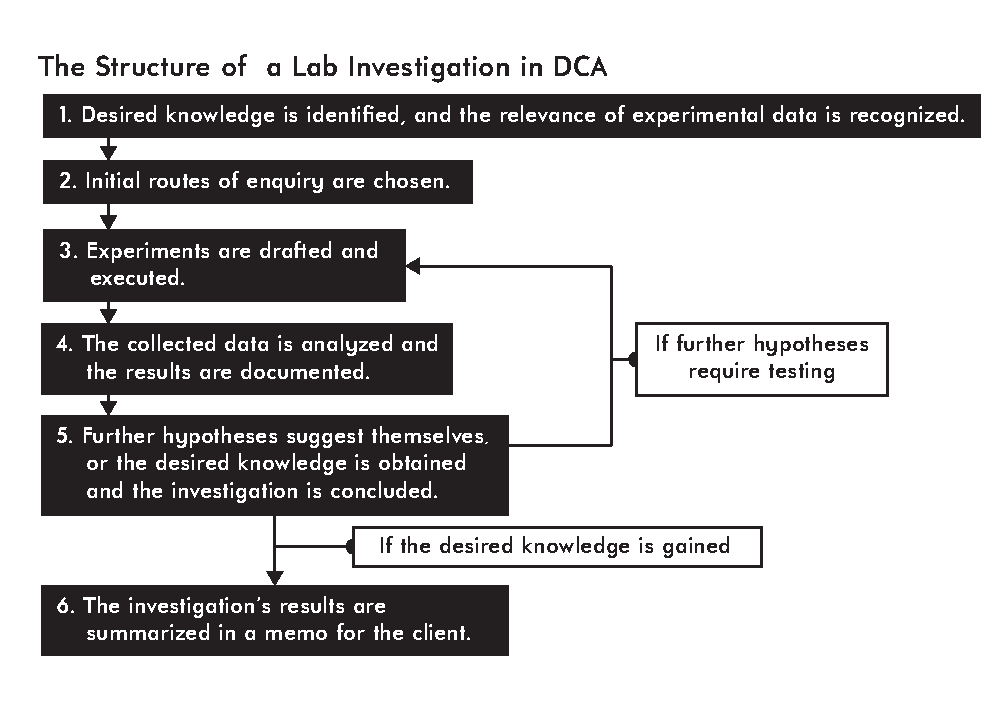
\includegraphics[width=1.2\textwidth]{Lab_Investigation_Diagram.pdf}
\caption{Investigation diagram.}
\label{fig:investigation_diagram}
\end{figure}


Applications of experimental design in engineering design include:
\begin{itemize}
\item Evaluation and comparison of basic design configurations
\item Evaluation of material alternatives
\item Selection of design parameters to produce a robust product
\item Determination of key product design parameters that impact performance
\end{itemize}
The use of experimental design in these areas can result in products that are easier to manufacture, have enhanced reliability and performance, lower product cost, and shorter product design and development time.
\par
Introducing experiment design at the concept stage could result in vastly better designs.

%%
\section{Experiment Design}
A designed experiment produces data that is relevant to the its objective and is logically unambiguous. An ``experiment design'' refers to the structure of an experiment, whereas ``Design of Experiments'' denotes both experiment designs and a broader philosophy of systematic experimentation.
\par
DCA's engineers are aware of the essentials of valid experimentation, these being:
\begin{description}
\item[Replication]{Testing a particular combination of factor levels with more than one unit. It allows us to estimate experimental error and to obtain a more precise estimate of a particular factor's influence.}
\item[Randomization]{Randomly determining the allocation of treatments to units and the sequence in which units are tested averages out the effects of nuisance variables, and validifies the assumption that units are randomly drawn from a particular distribution.}
\item[Blocking]{Accounting for possibly important differences between units when assigning treatments. A block is a set of similar units.}
\end{description}
Several experiment designs dominate in the company: 
\begin{description}
\item[Best-guess approach]{Factor levels for a test are chosen according to the results of a previous test. One or two factors at a time are varied in this way. \\ - No guarantee of optimal solution \\ - Can continue indefinitely.}
\item[One-factor-at-a-time]{A baseline set of factor levels are chosen, then each factor is varied across its range while all other factors are held at this baseline.\\ - Does not consider interactions \\ - Resource inefficient}
\item[Simple comparative]{}
\item[Factorial]{All possible combinations of factor levels are tested.}
\end{description}

Montgomery describes a traditional experiment design process as
\begin{enumerate}
\item Recognition and statement of the problem.
\item Choice of factors, levels, and ranges.
\item Selection of the response variable.
\item Choice of experimental design.
\item Performing the experiment.
\item Statistical analysis of the data.
\item Conclusions and recommendations.
\end{enumerate}
DCA certainly follow this structure, however it is implemented haphazardly across the company. For example, there is no formal guidance for steps 1-4, 6, or 7. This could result in several problems:
\begin{itemize}
\item Overlooking important properties of the problem at hand that may become apparent only when running an experiment, or that may not become apparent but would seriously influence interpretation of the data collected.
\item Neglecting to focus on aspects of the problem essential to the problem statement, because there is no formal problem statement to refer to.
\item Overlooking factors, or neglecting to set their levels/ranges in a systematic way. Choosing a non-optimal or irrelevant factor to modulate.
\item Choosing a sub-optimal response variable (i.e. one that has many degrees of separation between it and the phenomena of interest).
\item Choosing a resource-inefficient experiment design, or an experiment design that doesn't permit a desirable comparison in the analysis stage, or a design that fails to control for nuisance factors.
\item Incomplete identification of design or nuisance factors.
\item In general, pre-experimental planning is inadequate!
\item Choice of experimental design: sample size, run order, blocking or randomizatoin restrictions. 
\item Designing for analysis: analysis is typically minimal and kept extremely simple, with the exception of tests designed to British Standards.
\end{itemize}
The greatest strength of DCA's approach to its design of experiments is its simplicity. The designs are robust and the analyses are straightforward. It iterates on experiment designs until it is satisfied that they're adequate. Its biggest weaknesses are its inability to apply more sophisticated techniques when they are needed, and a haphazard monitoring of relevant problem factors. Examples of the former are lack of expertise handling resource-limited investigations and an inability to construct simple uncertainty measures on product parameters.
Certain documents must be kept for all experiments run - this means that raw data files, scans of handwritten observations, a table of the components used, and an Excel report summarizing the experiment's results must be produced and stored.
\par

%%
\section{Analysis}
Analyses in DCA consist of simple summary statistics and possibly use of classical hypothesis testing. The latter are informed by ISO 16269 (Statistical interpretation of data). This standard informs their construction of confidence and tolerance intervals, however their application within DCA is - in general - prescriptive. This section provides a short overview of simple summary statistics, then dissects the hypothesis tests detailed in ISO 16269.
\par
 A summary statistic is a value describes an aspect of a random variable's distribution. A random variable is a means of mapping physical events for which the outcome is uncertain to real numbers. For example, we could define a random variable $X$ that maps the outcomes of a coin toss onto the numbers 1 and 0:
 \begin{align}
	\texttt{Coin lands Heads} \implies X(s) = x = 1 \\
	\texttt{Coin lands Tails} \implies X(s) = x = 0
 \end{align}
In other words, $X$ is a function mapping from outcomes $s$ onto the real numbers $\mathbb{R}$, i.e. $X: s \mapsto \mathbb{R}$. Usually the mapping is quite natural - for example, we might use a random variable that denotes the number of sucesses in many trials, or the value of a measurement. Random variables are denoted with capital letters (e.g. $Y$) whereas the values they take on are lowercase letters (e.g. $y$).
\par
For summary statistics to be meaningful, it's necessary to understand the probability distributions that they describe. A probability distribution assigns probabilities to events. They can be either discrete or continuous: this distinction is important, as in the continuous case the probability of an r.v. taking on an exact value is zero (this is because any given interval over the real numbers of non-zero length contains infinitely many values). In the discrete case, the probability distribution takes the form of a probability mass function (PMF):
\[
	P(X = x) = f(x) : \sum_{-\infty}^{\infty} f(x) = 1; f(x) \geq 0
\]
If the random variable is continuous, then a probability density function is used to describe its probability distribution. A probability density can be thought of as the probability of a r.v. taking on a particular value if that value spanned a unit interval.
\[
	p(x) = f(x) : \int_{-\infty}^{\infty}f(x)\cdot dx = 1; f(x) \geq 1 \ \forall \ x
\]
To make the above two examples more concrete, consider the distributions shown in Figure \ref{fig:example_pd}.
\begin{figure}
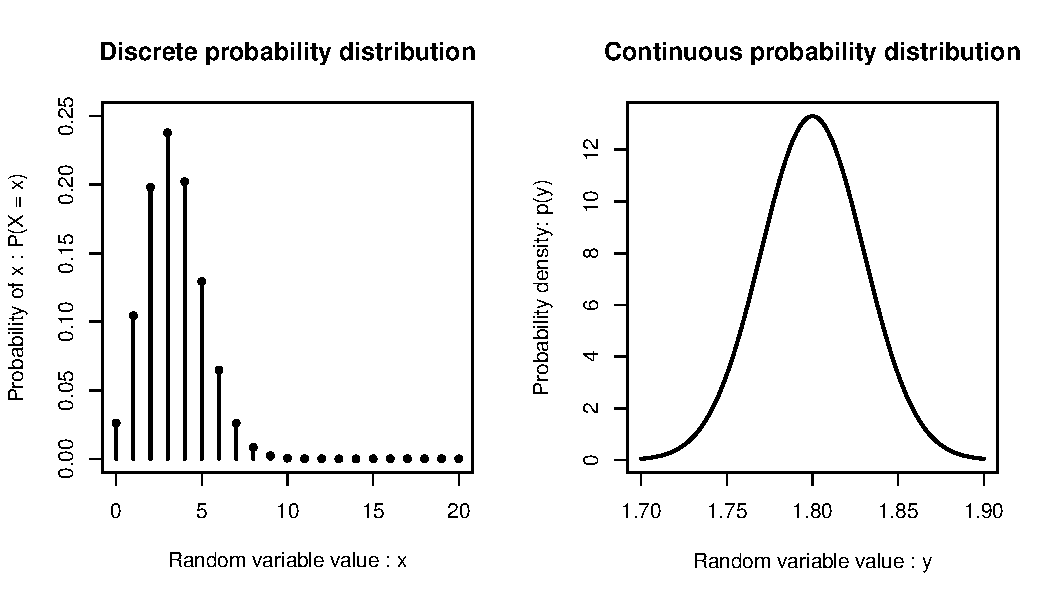
\includegraphics[width=\textwidth]{probability_distributions.pdf}
\label{fig:example_pd}
\caption{Probability mass and density functions are ways to express the probability distribution of discrete and continuous random variables.}
\end{figure}
 \par
All of this is relevant because summary statistics describe aspects of a probability distribution. The mean of a random variable, for example, summarizes the value at which the r.v.'s probability distribution is centered:
\[
	\mu = E[X] = \int_{-\infty}^{\infty}x\cdot p_X(x) \cdot dx
\]
Likewise, the variance of a random variable measures how spread out the r.v.'s probability distribution is:
\[
	\text{Var}X = E[(X - \mu)^2] = \int_{-\infty}^{\infty}(x - \mu)^2 \cdot p_X(x)\cdot dx
\]
The variance is average squared difference between a value that the r.v. can take on and the r.v.'s mean.
\par
A sample is a set of realizations of a random variable. Another way of saying this is that it's the result of a series of draws from the random variable's probability distribution. A sample can be used to infer the distribution of a random variable. One crude way of doing this is to draw from the distribution many times then chart the relative outcome frequencies. We can estimate a distribution's mean from a sample by computing the sample mean
\[
	\bar{X} = \frac{1}{n}\sum_{i = 1}^{n}x_i 
\]
It's possible to show that this will converge to the true mean as the sample size becomes very large. 
We can also estimate a distribution's variance from a sample. 
\begin{align}
	E[(X - \mu)^2] \ &= \ E[(\bar{X_n} - \mu)^2] + E[(X - \bar{X_n})^2]\\
	\sigma^2 \ &= \ \frac{\sigma^2}{n} +  \frac{1}{n}\sum_{i = 1}^n (X_i - \bar{X_n})^2 \\
	\implies \sigma^2 &= \frac{1}{n - 1}\sum_{i = 1}^{n}(X_i - \bar{X_n})^2
\end{align}
\par
DCA's most sophisticated statistical analysis is based on ISO 16269-6, \emph{Determination of statistical tolerance intervals}. This standard outlines how to construct tolerance intervals under either no assumptions about the random variable's distribution, or the assumption that the random variable has a normal distribution. A tolerance interval is a range of values that contain a particular fraction of the population to a given confidence level. A confidence level is the long-run proportion of intervals constructed that contain at least this proportion of the population. Consequently, tolerance intervals allow us to make statements about the performance of a population.
\par
The methods presented in ISO 16269-6 are presecriptive. The method they provide for computing the one-sided tolerance interval for a Normally distributed random variable of unknown mean and unknown standard deviation is as follows.
\par
We seek $k$ such that $\bar{x} + ks$ is greater than at least a proportion $p$ of the population with probability $1 - \alpha$. Let $\mu + u_p \sigma$ be greater than exactly a fraction $p$ of the population. Therefore:
\[
	P(\bar{x} + ks \geq \mu + u_p \sigma) = 1 - \alpha
\]
After some algebraic wrangling, it's possible to find:
\[
	P\Big(\frac{\sqrt{n}(\sigma u_p - \bar{x} + \mu)}{s} \leq \sqrt{n}k\Big) = 1 - \alpha
\]
The term on the l.h.s. of the inequality has a t-distribution with $n - 1$ degrees of freedom and location $\sqrt{n}u_p$. This means that 
\[
	\sqrt{n}k = t_{1 - \alpha}(\sqrt{n}u_p, n - 1)
\]
where $t_{1 - \alpha}(...)$ is the value corresponding to the $1 - \alpha$ percentile of the t-distribution with $n - 1$ degrees of freedom centered at $\sqrt{n}u_p$. The interval containing at least $p$ of the population with probability $1 - \alpha$ is therefore:
\[
	\Big(-\infty, \bar{x} + \frac{t_{1 - \alpha}(\sqrt{n}u_p, n - 1)\cdot s}{\sqrt{n}}\Big]
\]
This interval contains at least a fraction $p$ of the population with probability $1 - \alpha$. Example tolerance intervals are shown in Figure \ref{fig:tolerance_intervals}.
\begin{figure}
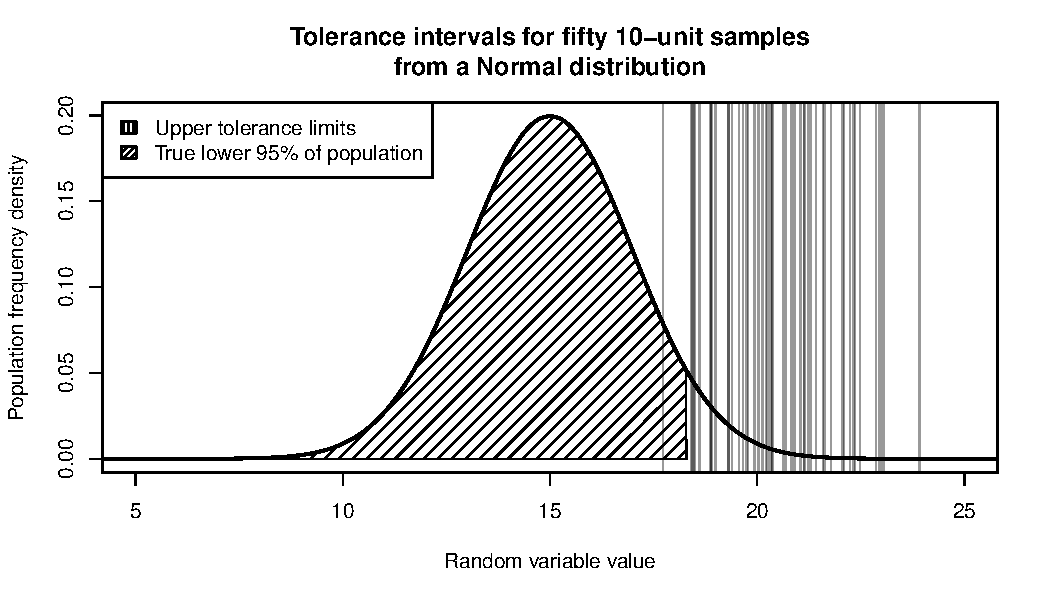
\includegraphics[width=\textwidth]{tolerance_intervals.pdf}
\caption{Example tolerance limits for a confidence level of 0.95. Each vertical line corresponds to a 95\% tolerance limit constructed for a simulated 10-unit sample.}
\label{fig:tolerance_intervals}
\end{figure}
At present, DCA do not test the assumption of Normality (check this).
% Questions:
%	> What is a t-distribution?
% 	> Do DCA test the normality assumption?
%	> 
\par
% Confidence intervals
Another tool that DCA's engineers occasionally use is confidence intervals. A confidence interval contains the value of a population parameter a proportion 1 - $\alpha$ of the cases in a long series of repeated random samples under identical conditions. They're useful when we want to quantify the uncertainty on our estimate of a population parameter such as the mean or variance. Again, these are applied in a presciptive manner, and the underlying assumptions are rarely checked. Rather than give a derivation of them here, they're suspended until Section X where they're shown in the context of Bayesian inference.
\par
% Two-sample t-tests
THE FOLLOWING PLAGIARIZES MONTGOMERY AND SHALL BE CHANGED
Occasionally an analysis of a comparative test will contain a two-sample t-test. This assumes that the variances of the two groups tested is the same (i.e. the treatment may only affect the group mean, not its variance), and that the samples are randomly drawn from the same Normal distribution. The $p$-value obtained corresponds to the probability of observing the difference in sample means assuming that the two samples were drawn from the same Normal distribution. The implication of a small $p$-value is that assuming the two samples were drawn from the same Normal distribution is unreasonable. The two-sample t-test statistic is
\[
	t_0 = \frac{\bar{y}_1 - \bar{y}_2}{s_p^2 \cdot \sqrt{\frac{1}{n_1} + \frac{1}{n_2}}}
\]
Where $s_p^2$ is an estimate of the the two group's common variance $\sigma^2$:
\[
	s_p^2 = \frac{(n_1	 - 1)\cdot s_1^2 + (n_2 - 1)\cdot s_2^2}{n_1 + n_2 - 2}	
\]
If $t_0$ were greater than the value of t corresponding to the $\alpha/2$ percentage point of the t distribution with $n_1 + n_2 - 2$ degrees of freedom, we would reject $H_0$ and conclude that the means of the two groups differ.
\par
If we are sampling from independent Normal distributions, the the distribution of $\bar{y}_1 - \bar{y}_2$ is $N(\mu_1 - \mu_2, \sigma^2(1/n_1 + 1/n_2))$. Thus if the two distributions shared the same mean, then
\[
	Z_0 = \frac{\bar{y}_1 - \bar{y}_2}{\sigma\sqrt{\frac{1}{n_1} + \frac{1}{n_2}}}
\]
would be a $N(0, 1)$ r.v. However, because $\sigma$ is unknown, we must instead replace it with an estimate of the population standard deviation $s_p$, resulting in an r.v. that has a t-distribution.
\newpage
% Monte Carlo simulation
Monte Carlo simulation approximates a quantity by simulating the random process generating it . It has previously been applied within DCA to understand SOMETHING. The use case was somewhat similar to the following: the expectation of some analytically inconvenient function of a random variable was needed. Take $Y \sim \text{Binom}(n = 10, p = X)$ as an example, where $X \sim \text{Beta}(a = 7, b = 3)$\footnote{The beta distribution is a continuous and generates a number between $0$ and $1$, which makes it useful in modelling the distribution of a probability.}. Rather than calculate the expectation directly, tens of thousands of values of $y$ were generated according to $Y$'s distribution using a computer. Each of these values were then used to randomly generate a value of $x$ from $\text{Binom}(n = 10, p = y)$. The resulting frequencies of the $x$ values then represented $X$'s distribution. It was then possible to calculate the mean by averaging over all the $x$ values obtained. A diagram of this process is shown in Figure \ref{fig:monte_carlo}.
\begin{figure}
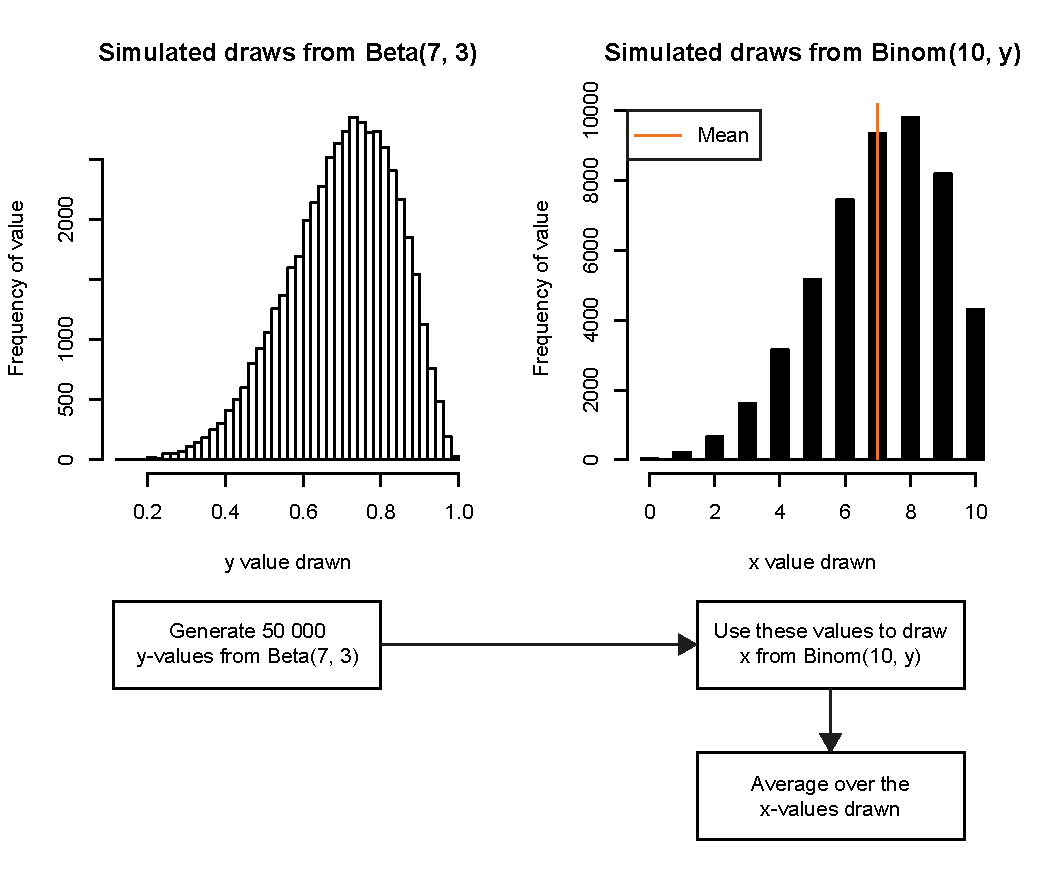
\includegraphics[width=\textwidth]{monte_carlo_simulation.pdf}
\label{fig:monte_carlo}
\caption{Process diagram for a Monte Carlo simulation.}
\end{figure}



\subsection{Visualization}
DCA's reports and client presentations frequently contain plots of the data collected from an experiment. These plots are almost exclusively either line charts or scatter plots generated using Microsoft Excel. 
\par
A summary line chart would consist of many independent unit's results overlaid, such that a visual comparison of two groups would look similar to Figure \ref{fig:line_plots}.
\begin{itemize}
\item[+] Allows an entire test to be viewed simultaneously, providing a high-level summary of the results
\item[-] Obscures the behaviour of individual units
\item[-] Makes it unclear whether the results are from separate units or not
\item[-] Encourages experimenter to focus on extreme cases, rather than overall performance
\item[-] Obscures differences between groups that aren't related to location or dispersion (such as harmonic content)
\end{itemize}
\begin{figure}[b!]
	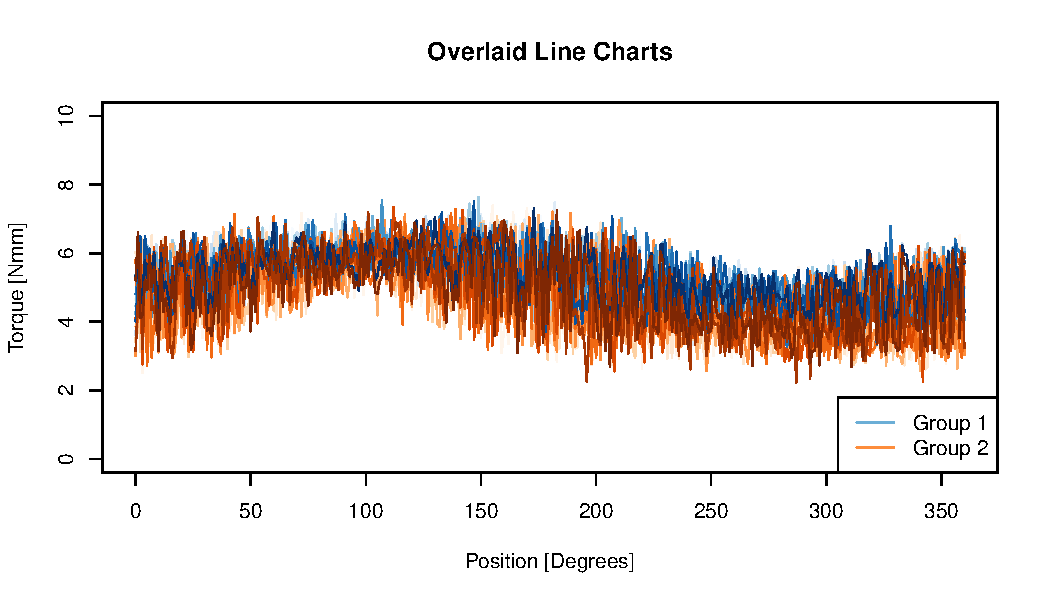
\includegraphics[width=\textwidth]{overlaid_line_charts.pdf}
	\label{line_plots}
	\caption{Sample summary line chart from a DCA test report.}
\end{figure}
DCA pair a visualization with the tolerance intervals in the preceding section.
EXAMPLE TOLERANCE INTERVAL PLOT

%% MEDICAL INDUSTRY'S USE OF STATISTICS %%
\chapter{Overview of the Medical Industry's Use of Statistics}\label{industry_context} %% CONTEXT %%

\section{Experiment Design}

\section{Analysis}
\subsection{Exploratory Analysis}
\subsection{Descriptive Analysis}
\subsection{Inferential Analysis}

\section{Presentation \& Visualization}

\section{Summary}

\newpage


%% PROPOSED METHODS %%
\chapter{Suggested Methods}
%%
\section{Design of Experiments}
\subsection{Blocking}
\subsection{Factorial designs}
\subsection{Taguchi}
\subsection{Strategies for handling limited sample sizes}

%%
\section{Analysis}
\subsection{Sumary Statistics}
\subsection{Regression Models}
Regression models are a flexible tool that allow us to
\begin{itemize}
\item Estimate the effects of discrete and continuous factors on a unit's response - even if they interact or have a nonlinear influence.
\item Identify differences between units that aren't immediately apparent from raw data
\item Measure how well our understanding of a product lines up with its reality
\end{itemize}
\subsection{Bayesian Inference}
\subsection{Markov Chain Simulation}

%%
\section{Presentation \& Visualization}
\subsection{The Psychology of a Plot}
\subsection{Scatter plots}
\subsection{Histograms}
\subsection{Box plots}
\subsection{Separation Plots}
http://mdwardlab.com/sites/default/files/GreenhillWardSacks.pdf

%%
\section{Software}
\begin{itemize}
\item Excel
\item Matlab
\item R
\item Python
\item Minitab
\end{itemize}

\newpage


%% CONCLUSIONS AND RECOMMENDATIONS %%
\chapter{Conclusions \& Recommendations}

\newpage
\appendix
\chapter{}
Probability allows us to analyze a system without requiring complete mechanical knowledge of it. `'Randomness'' refers to sources of variation that aren't measured. You may have heard of probabilities as representing `'Degrees of belief''. To understand what a belief is, consider this example. We machine a coin that we check is a symmetric disk of homogeneous density. I flip the coin ten times, and it comes up heads every single time. You might be surprised by this, and accuse me of flipping it in a controlled way. I then ask you how I can flip it in a way that is fair. What is your response?
\par
If you say that it should come heads as many times as tails, then the experiment is no longer random, as we know what the outcome will be. You may gesticulate and say ``You need to flip it \emph{randomly}''. I would press you to tell me what this means - I require a mechanism to decide how to flip the coin, and physical mechanisms are deterministic.
\par
The probability of an outcome can only be evaluated to a set of assumptions you make about the mechanism generating those outcomes. You had a preconceived notion that the way I flipped the coin would favor neither heads nor tails, and therefore saw ten heads as supremely improbable.

% Ronald Fisher, The Design of Experiments
% Attacking the interpretation or data collection method
% `an experimenter... wishes to safeguard his results, ... from ignroant criticism by different sorts of superior persons'
% Criticizes Bayes' theorem: ` Advocates of inverse probability seem forced to regard mathematical probability not as an
%					objective quantity measured by observable frequencies, but as measureent merely
%					psychological tendencies'
% `Experimental observations are only experience planned in advance, and designed to form a secure basis of new knowledge'
% Refs: 	- An essay towards solving a problem in the doctrine of chances, T. Bayes (1763)

% R. Mead, Design of Experiments
% Introduction
% ---------------
% - Degrees of freedom - count of the number of independent comparisons that can be made
% - The total information in an experiment involving N experiental units may be represented by the total variation based on N -1 df
%		> Variation is divided into three components:
%			- Treatment component T, sum of df corresponding to the questions to be asked
%			- Blocking component B, representing all environment effects that are to be included in the fitted model.
%			  (b - 1)df for b blocks.
%			-  Error component E, used to estimate the error's variance (i.e. estimate the standard errors)
%	The resource equation:	T + B + E = N - 1
%	To obtain a good estimate of error, need at least 10 df (preferably 15)
%	- Calculable by examining the 5% point of the t-distribution, and using enough df that increasing the error df
%	  makes little difference to the significance value.
%
% One final comment on this question of efficient use of resources. It is, of course, possible
% to keep the value of E in the region of 10–20 by doing several small experiments, rather than
% one rather larger experiment in which the total number of experimental units is much less
% than the sum of the units in the separate small experiments. This is inefficient because of the
% need to estimate σ2 for each separate experiment. Experimenters should identify clearly the
% questions they wish the experiment to cover, and they should also consider carefully if they
% are asking enough questions to use the experimental resources efficiently.

% Randomized complete block design: Essentially each group of ‘similar’ units
%					        should include roughly equal numbers of units for each treatment. 
%					        This control is referred to as blocking.
%						- `Similar' units -> e.g. same spring orientation, batch numbers, cavity numbers
%					       Each block contains a single replicate of each of the treatments.
%					       Key idea is to make groups subject to similar sources of variation.
%					      A `block' is a group of similar units.
% Completely randomized design: Randomly allocate treatments to units.
%

% Analysis of variance
% - Provides a subdivision of the total variation between the exerimental units into separate components, each component
%	representing a different source of variation, so that the relative importance of the different sources can be assessed.
% - Gives and estimate of the underlying variation between units, providing a basis for inferences about the applied
%	treatments.
% The basic philosophy of analysis of variance is to assume that each unit has an inherent
% response, possibly related to the position of the unit within the experiment, which is modified
% by the effect of the particular treatment applied to the unit.
% Response in terms of components y_{ij} = \mu + b_i + t_j _ \epsilon_{ij}
% \mu is the average of the whole set of experimental units, b_i is the term representing the average deviation
% from \mu of the units in block i, t_j is the term representing the average deviation from the \mu of the units given treatment j,
% \epsilon_{ij}  represents the deviation of a particular unit from \mu + b_i.
% sum over t_j must equal zero, as must the sum over b_i.
% Assumptions: - Individual unit variation is not affected by treatment applied to the unit.
%		      - The effect of each treatment is additive - the chosen block does not affect the efficacy of the treatment.
% The analysis of variance of data from an experimental design is simply the division of the
% total variation between the n observations into sensibly distinguishable components, and the
% subsequent interpretation of the relative size of the components
% Applying this principle to the randomized block design, we get
% \[
%	total SS = block SS + treatment SS + error SS
% \]
% Standard error of the difference between treatments
% In addition, it is natural, when making comparisons, to concentrate on
% those comparisons which look larger, which will be between the treatments giving the more
% extreme results and which are then subject to a selection bias.n addition, it is natural, when making comparisons, to concentrate on
% those comparisons which look larger, which will be between the treatments giving the more
% extreme results and which are then subject to a selection bias.

% Multiple blocking and recording of nuisance variables
\end{document}